\documentclass{article}

% Additional packages & macros
\usepackage[a4paper, margin=1in]{geometry}
\usepackage{fancyhdr}
\pagestyle{fancy}
\usepackage{minted}
\usepackage{xcolor}
\usemintedstyle{pastie}
\usepackage{booktabs}     % For cleaner tables (\toprule, \midrule, \bottomrule)
\usepackage{amsmath}      % General maths support
\usepackage{amssymb}      % Additional maths symbols
\usepackage{graphicx}     % If you're including any images
\usepackage{hyperref}     % For clickable links (if needed)
\usepackage{tikz}
\usetikzlibrary{positioning}
\usepackage{tcolorbox}
\tcbuselibrary{listingsutf8}
\definecolor{mintgreen}{rgb}{0.95,1,0.95} % soft green to match Pastie
\newcommand{\codecmd}[1]{\textcolor[rgb]{0,0.5,0}{\texttt{#1}}}
\usepackage{float}

% Header and footer
% ! Unit name
\newcommand{\unitName}{CAB302 Software Development}
% ! Unit semester 
\newcommand{\unitTime}{Semester 2, 2025}
% ! Unit coordinator name
\newcommand{\unitCoordinator}{Unit Coordinator: Alessandro Soro}
% ! Document authors
\newcommand{\documentAuthors}{Monica Borg}

\fancyhead[L]{\unitName}
\fancyhead[R]{\leftmark}
\fancyfoot[C]{\thepage}

\date{}

\begin{document}
%
\begin{titlepage}
    \vspace*{\fill}
    \begin{center}
        \LARGE{\textbf{\unitName}} \\[0.1in]
        \normalsize{\unitTime} \\[0.2in]
        \normalsize\textit{\unitCoordinator} \\[0.2in]
        \documentAuthors
    \end{center}
    \vspace*{\fill}
    \thispagestyle{empty}
\end{titlepage}
\newpage
%
\tableofcontents
\newpage
%
\section{Object Oriented Programming with Java}

\subsection{Java}
Java is a high-level, class-based, object-oriented programming language that is platform-independent and widely used for developing applications across desktop, web, and mobile environments. It follows the syntax and structure of the C-family of languages, making it familiar to developers with experience in C or C\#.

Originally created in the 1990s at Sun Microsystems, Java was designed to be platform-independent and architecture-neutral, enabling code to run consistently across various systems (regardless of endianness\footnote{Endianness, in computing, refers to the order in which bytes within a word of digital data are stored in computer memory or transmitted over a network. It can be either big-endian (most significant byte first) or little-endian (least significant byte first)}). Java supports automatic garbage collection, offers robust memory management, and was developed with the internet in mind. Since becoming open source in 2006, it has served as the primary platform for Android development.

A basic Java program includes a class definition and a \codecmd{main} method, which serves as the entry point for execution. For example, a program that prints \codecmd{Hello, world!} to the console can be written as:

\begin{minted}[fontsize=\small, linenos, breaklines]{java}
public class HelloWorld {
    public static void main(String[] args) {
        System.out.println("Hello, world!");
    }
}
\end{minted}

\subsection{Primitive Data Types in Java}
Java provides a set of built-in primitive data types for representing simple values. These types are not objects and form the most basic elements for data representation and manipulation:

\begin{table}[h!]
\centering
\begin{tabular}{@{}lll@{}}
\toprule
\textbf{Type} & \textbf{Size} & \textbf{Description} \\
\midrule
\texttt{byte}   & 8-bit   & Signed two’s complement integer. Range: \texttt{-128} to \texttt{127} \\
\texttt{short}  & 16-bit  & Signed two’s complement integer. Range: \texttt{-32,768} to \texttt{32,767} \\
\texttt{int}    & 32-bit  & Signed two’s complement integer. Range: \texttt{-2,147,483,648} to \texttt{2,147,483,647} \\
\texttt{long}   & 64-bit  & Signed two’s complement integer. Range: \texttt{-9,223,372,036,854,775,808} \\
                &         & to \texttt{9,223,372,036,854,775,807} \\
\texttt{float}  & 32-bit  & IEEE 754 single-precision floating point \\
\texttt{double} & 64-bit  & IEEE 754 double-precision floating point \\
\texttt{boolean}& 1-bit*  & Represents \texttt{true} or \texttt{false} \\
\texttt{char}   & 16-bit  & A single Unicode character \\
\bottomrule
\end{tabular}
\end{table}
\textit{*\textbf{Note}: The size of a \codecmd{boolean} is not fixed and depends on the JVM implementation. It is often 1 byte but not guaranteed.}

\subsection{Java Operators}

\subsubsection{Arithmetic Operators}
\begin{center}
\begin{tabular}{@{}lll@{}}
\toprule
\textbf{Operator} & \textbf{Name} & \textbf{Example} \\
\midrule
\texttt{+}  & Addition       & \texttt{x + y} \\
\texttt{-}  & Subtraction    & \texttt{x - y} \\
\texttt{*}  & Multiplication & \texttt{x * y} \\
\texttt{/}  & Division       & \texttt{x / y} \\
\texttt{\%} & Modulus        & \texttt{x \% y} \\
\texttt{++} & Increment      & \texttt{++x} \\
\texttt{--} & Decrement      & \texttt{--x} \\
\bottomrule
\end{tabular}
\end{center}

\vspace{1em}
\subsubsection{Assignment Operators}
\begin{center}
\begin{tabular}{@{}lll@{}}
\toprule
\textbf{Operator} & \textbf{Example} & \textbf{Equivalent To} \\
\midrule
\texttt{=}    & \texttt{x = 5}    & \texttt{x = 5} \\
\texttt{+=}   & \texttt{x += 3}   & \texttt{x = x + 3} \\
\texttt{-=}   & \texttt{x -= 3}   & \texttt{x = x - 3} \\
\texttt{*=}   & \texttt{x *= 3}   & \texttt{x = x * 3} \\
\texttt{/=}   & \texttt{x /= 3}   & \texttt{x = x / 3} \\
\texttt{\%=}  & \texttt{x \%= 3}  & \texttt{x = x \% 3} \\
\texttt{\&=}  & \texttt{x \&= 3}  & \texttt{x = x \& 3} \\
\texttt{|=}   & \texttt{x |= 3}   & \texttt{x = x | 3} \\
\texttt{\^=}  & \texttt{x \^= 3}  & \texttt{x = x \^ 3} \\
\texttt{>>=}  & \texttt{x >>= 3}  & \texttt{x = x >> 3} \\
\texttt{<<=}  & \texttt{x <<= 3}  & \texttt{x = x << 3} \\
\bottomrule
\end{tabular}
\end{center}

\vspace{1em}
\subsubsection{Logical Operators}
\begin{center}
\begin{tabular}{@{}lll@{}}
\toprule
\textbf{Operator} & \textbf{Name} & \textbf{Example} \\
\midrule
\texttt{\&\&} & Logical AND & \texttt{x < 5 \&\& x < 10} \\
\texttt{||}  & Logical OR  & \texttt{x < 5 || x < 4} \\
\texttt{!}   & Logical NOT & \texttt{!(x < 5 \&\& x < 10)} \\
\bottomrule
\end{tabular}
\end{center}

\vspace{1em}
\subsubsection{Comparison Operators}
\begin{center}
\begin{tabular}{@{}lll@{}}
\toprule
\textbf{Operator} & \textbf{Name} & \textbf{Example} \\
\midrule
\texttt{==} & Equal to                 & \texttt{x == y} \\
\texttt{!=} & Not equal                & \texttt{x != y} \\
\texttt{>}  & Greater than             & \texttt{x > y} \\
\texttt{<}  & Less than                & \texttt{x < y} \\
\texttt{>=} & Greater than or equal to & \texttt{x >= y} \\
\texttt{<=} & Less than or equal to    & \texttt{x <= y} \\
\bottomrule
\end{tabular}
\end{center}

\subsubsection{Operator Overloading}

Java does \textbf{not support operator overloading}. This means the behaviour of standard operators (e.g., \texttt{+}, \texttt{-}) cannot be redefined for user-defined types such as classes.

\subsection{Object-Oriented Principles in Java}

Java’s object-oriented paradigm is based on four core principles:

\begin{itemize}
    \item \textbf{Encapsulation} – Data (fields) and behaviour (methods) are combined into classes. Internal state is protected using access modifiers.
    \item \textbf{Abstraction} – Interface definitions and abstract classes allow internal implementation to be hidden while exposing only essential behaviour.
    \item \textbf{Inheritance} – A class can inherit from another to reuse properties and behaviour via the \texttt{extends} keyword.
    \item \textbf{Polymorphism} – Method behaviour can vary depending on the runtime object type, achieved via overriding and interfaces.
\end{itemize}

\subsubsection{Everything's an Object}

In Java, \codecmd{java.lang.Object} is the ultimate superclass of all classes. Every Java object (including arrays) inherits its methods. These include:

\begin{itemize}
    \item \codecmd{clone()} – Returns a copy of the object (shallow copy).
    \item \codecmd{equals(Object obj)} – Compares for equality.
    \item \codecmd{hashCode()} – Generates a hash code for use in hash tables.
    \item \codecmd{toString()} – Returns a string representation of the object.
    \item \codecmd{getClass()} – Provides the object's runtime class.
    \item \codecmd{finalize()} – Invoked by the garbage collector before destruction.
    \item \codecmd{wait()}, \codecmd{notify()}, \codecmd{notifyAll()} – Used for thread coordination.
\end{itemize}

These methods form the core behaviours available to every Java object.

\smallskip
\textit{See:} \href{https://docs.oracle.com/javase/8/docs/api/java/lang/Object.html}{\texttt{docs.oracle.com/javase/8/docs/api/java/lang/Object.html}}

\subsection{Foundational Java Features}

This section outlines core language features in Java that support structured program development and object-oriented design.

\subsubsection{Classes}

Classes serve as templates for defining objects, encapsulating both data and behaviour. Each class may define fields, methods, and constructors to manage its internal state and expose functionality.

\begin{minted}[fontsize=\small, linenos, breaklines]{java}
class Person {
    private String name;

    public Person(String name) {
        this.name = name;
    }

    public void greet() {
        System.out.println("Hello, " + name + "!");
    }
}
\end{minted}

While classes are fundamental to object-oriented design, \hyperref[subsec:interfaces]{interfaces} are often preferred when defining shared behaviour across unrelated types. Java supports only single inheritance for classes, meaning a class can extend only one superclass. In contrast, interfaces allow multiple inheritance of type, enabling a class to implement multiple interfaces. This promotes greater flexibility, modularity, and adherence to the principle of programming to an interface rather than to an implementation.



\subsubsection{Constructors and Encapsulation}

Constructors are used to initialise objects when they are created. Encapsulation ensures internal fields are kept private, with controlled access provided through methods (getters and setters).

\begin{minted}[fontsize=\small, linenos, breaklines]{java}
class BankAccount {
    private double balance;

    public BankAccount(double initialBalance) {
        balance = initialBalance;
    }

    public double getBalance() {
        return balance;
    }

    public void deposit(double amount) {
        if (amount > 0) {
            balance += amount;
        }
    }
}
\end{minted}

\subsubsection{Command Line Arguments}

Command line arguments are passed to Java applications through the \codecmd{main} method. These values can be used to modify program behaviour at runtime.

\begin{minted}[fontsize=\small, linenos, breaklines]{java}
public class ArgumentPrinter {
    public static void main(String[] args) {
        if (args.length > 0) {
            System.out.println("First argument: " + args[0]);
        } else {
            System.out.println("No arguments provided.");
        }
    }
}
\end{minted}

\subsubsection{Standard Output}

Output to the console is typically performed using \codecmd{System.out.print()} and \codecmd{System.out.println()}. These are commonly used for program feedback and debugging.

\begin{minted}[fontsize=\small, linenos, breaklines]{java}
public class OutputExample {
    public static void main(String[] args) {
        System.out.print("This is printed on the same line. ");
        System.out.println("This ends with a newline.");
    }
}
\end{minted}


\subsection{Using Interfaces in Java for OOP}
\label{subsec:interfaces}

In Java, an \codecmd{interface} defines a set of method signatures that implementing classes must fulfil. This promotes abstraction and allows different classes to share common behaviour without enforcing inheritance.

Interfaces may contain:
\begin{itemize}
    \item Abstract methods (implicitly \codecmd{public abstract})
    \item \codecmd{default} methods with implementation
    \item \codecmd{static} methods
    \item Constants (\codecmd{public static final})
\end{itemize}

Classes implement interfaces using the \codecmd{implements} keyword. All abstract methods must be defined by the implementing class.

Interfaces are preferred in Java over class inheritance when designing for flexibility and modularity. Since Java does not support multiple class inheritance, interfaces offer a mechanism for multiple behavioural inheritance. This approach avoids the fragility associated with deep inheritance hierarchies and encourages composition over inheritance. It also enables different classes to share a common set of behaviours without enforcing a shared ancestry.


\subsubsection*{Example: Interface \& Implementation}

\begin{minted}[fontsize=\small, linenos, breaklines]{java}
interface Animal {
    void makeSound(); // abstract method
}

class Dog implements Animal {
    public void makeSound() {
        System.out.println("Woof!");
    }
}

class Cat implements Animal {
    public void makeSound() {
        System.out.println("Meow!");
    }
}

public class Main {
    public static void main(String[] args) {
        Animal a1 = new Dog();
        Animal a2 = new Cat();
        a1.makeSound(); // Woof!
        a2.makeSound(); // Meow!
    }
}
\end{minted}

This example demonstrates \textbf{polymorphism} through interface references. Both \codecmd{Dog} and \codecmd{Cat} implement \codecmd{Animal}, enabling uniform handling while invoking class-specific behaviour.

\subsubsection*{Example: Interface with Multiple Implementations in a Strategy Pattern}

Interfaces can support behavioural flexibility by enabling interchangeable algorithms. In the example below, an interface is used to encapsulate different payment strategies.

\begin{minted}[fontsize=\small, linenos, breaklines]{java}
interface PaymentStrategy {
    void pay(int amount);
}

class CreditCardPayment implements PaymentStrategy {
    public void pay(int amount) {
        System.out.println("Paid $" + amount + " with credit card.");
    }
}

class PayPalPayment implements PaymentStrategy {
    public void pay(int amount) {
        System.out.println("Paid $" + amount + " using PayPal.");
    }
}

class Checkout {
    private PaymentStrategy strategy;

    public Checkout(PaymentStrategy strategy) {
        this.strategy = strategy;
    }

    public void processPayment(int amount) {
        strategy.pay(amount);
    }
}

public class Main {
    public static void main(String[] args) {
        Checkout c1 = new Checkout(new CreditCardPayment());
        c1.processPayment(100);

        Checkout c2 = new Checkout(new PayPalPayment());
        c2.processPayment(200);
    }
}
\end{minted}

This demonstrates the \textbf{Strategy Pattern}, where interchangeable implementations of \codecmd{PaymentStrategy} are used at runtime. This decouples the client class (\codecmd{Checkout}) from specific implementations.

\subsubsection*{Example: Interface Inheritance and Default Methods}

Interfaces in Java can extend other interfaces and also provide default method implementations.

\begin{minted}[fontsize=\small, linenos, breaklines]{java}
interface Shape {
    double area();
}

interface Printable {
    default void print() {
        System.out.println("Printing shape...");
    }
}

class Circle implements Shape, Printable {
    private double radius;

    public Circle(double radius) {
        this.radius = radius;
    }

    public double area() {
        return Math.PI * radius * radius;
    }

    // Optional: override default print
    public void print() {
        System.out.println("Circle with area: " + area());
    }
}

public class Main {
    public static void main(String[] args) {
        Circle c = new Circle(3.0);
        c.print(); // Circle with area: 28.27...
    }
}
\end{minted}

This example illustrates:
\begin{itemize}
    \item Multiple interface implementation (\codecmd{Shape} and \codecmd{Printable})
    \item Use and override of a \codecmd{default} method
    \item Compositional design via behaviour-based contracts
\end{itemize}

\medskip
\textit{Using interfaces in this way supports a clean separation of concerns and promotes reusable, modular design.}


\medskip
\textit{Interfaces are well suited for defining contracts that can be shared across unrelated classes.}

\subsection{Object-Oriented Libraries in Java}

The Java Standard Library includes a comprehensive collection of packages built on object-oriented principles. These libraries provide reusable classes for data structures, file I/O, networking, time manipulation, and system interaction.

\subsubsection*{java.util}

This package provides utility classes including collections, data structures, random number generation, and date/time classes.

\begin{itemize}
    \item \codecmd{ArrayList} – A dynamically resizing array.
    \item \codecmd{HashMap} – A key-value data structure with constant-time lookup.
    \item Additional utilities include \codecmd{LinkedList}, \codecmd{HashSet}, \codecmd{Date}, \codecmd{Calendar}, and \codecmd{Random}.
\end{itemize}

\noindent\textbf{Example: Using \codecmd{ArrayList} and \codecmd{HashMap}}
\begin{minted}[fontsize=\small, linenos, breaklines]{java}
import java.util.ArrayList;
import java.util.HashMap;

public class UtilExample {
    public static void main(String[] args) {
        ArrayList<String> names = new ArrayList<>();
        names.add("Alice");
        names.add("Bob");

        HashMap<String, Integer> scores = new HashMap<>();
        scores.put("Alice", 85);
        scores.put("Bob", 90);

        System.out.println("Names: " + names);
        System.out.println("Bob's score: " + scores.get("Bob"));
    }
}
\end{minted}

\subsubsection*{java.io}

Provides classes for input/output streams, file access, character encoding, and buffered I/O operations.

\begin{itemize}
    \item \codecmd{File}, \codecmd{FileReader}, \codecmd{FileWriter}
    \item \codecmd{BufferedReader}, \codecmd{PrintWriter}
    \item \codecmd{InputStream}, \codecmd{OutputStream}
\end{itemize}

\noindent\textbf{Example: Writing to and reading from a file}
\begin{minted}[fontsize=\small, linenos, breaklines]{java}
import java.io.*;

public class IOExample {
    public static void main(String[] args) throws IOException {
        // Write to file
        PrintWriter writer = new PrintWriter("example.txt");
        writer.println("Hello, file!");
        writer.close();

        // Read from file
        BufferedReader reader = new BufferedReader(new FileReader("example.txt"));
        String line = reader.readLine();
        System.out.println("Read: " + line);
        reader.close();
    }
}
\end{minted}

\subsubsection*{java.net}

This package enables network communication using sockets, IP addresses, and URLs.

\begin{itemize}
    \item \codecmd{Socket}, \codecmd{ServerSocket}
    \item \codecmd{URL}, \codecmd{URLConnection}
    \item \codecmd{InetAddress}
\end{itemize}

\noindent\textbf{Example: Accessing a web page using \texttt{URL}}
\begin{minted}[fontsize=\small, linenos, breaklines]{java}
import java.net.*;
import java.io.*;

public class NetworkExample {
    public static void main(String[] args) throws Exception {
        URL url = new URL("https://example.com");
        BufferedReader reader = new BufferedReader(
            new InputStreamReader(url.openStream()));
        String line;
        while ((line = reader.readLine()) != null) {
            System.out.println(line);
        }
        reader.close();
    }
}
\end{minted}

\subsubsection*{java.lang}

Contains essential classes such as \codecmd{Object}, \codecmd{System}, \codecmd{Math}, and wrapper types. It is automatically imported into every Java program.

\begin{itemize}
    \item \codecmd{Object} – Superclass of all Java classes
    \item \codecmd{System} – Access to standard input/output and system properties
    \item \codecmd{Math}, \codecmd{String}, \codecmd{Integer}, etc.
\end{itemize}

\noindent\textbf{Example: Using \texttt{System} and \texttt{Math}}
\begin{minted}[fontsize=\small, linenos, breaklines]{java}
public class LangExample {
    public static void main(String[] args) {
        System.out.println("Square root of 64 is: " + Math.sqrt(64));
        System.out.println("Available memory: " + Runtime.getRuntime().freeMemory());
    }
}
\end{minted}

\subsubsection*{java.time}

Introduced in Java 8, this package provides a modern date and time API with immutable and thread-safe classes.

\begin{itemize}
    \item \codecmd{LocalDate}, \codecmd{LocalTime}, \codecmd{LocalDateTime}
    \item \codecmd{Duration}, \codecmd{Period}, \codecmd{ZoneId}, \codecmd{ZonedDateTime}
    \item Preferred over \codecmd{java.util.Date} and \codecmd{Calendar} for new development
\end{itemize}

\noindent\textbf{Example: Working with dates and times}
\begin{minted}[fontsize=\small, linenos, breaklines]{java}
import java.time.LocalDate;
import java.time.LocalTime;
import java.time.LocalDateTime;

public class TimeExample {
    public static void main(String[] args) {
        LocalDate date = LocalDate.now();
        LocalTime time = LocalTime.now();
        LocalDateTime dateTime = LocalDateTime.now();

        System.out.println("Date: " + date);
        System.out.println("Time: " + time);
        System.out.println("DateTime: " + dateTime);
    }
}
\end{minted}

\subsubsection*{java.nio.file}

This package is part of the NIO.2 API and provides advanced file and directory handling with improved performance and flexibility.

\begin{itemize}
    \item \codecmd{Files} – Static methods for file operations (e.g., copy, move, delete)
    \item \codecmd{Paths}, \codecmd{Path} – Represent file and directory locations
    \item Supports symbolic links, file attributes, and stream-based file access
\end{itemize}

\noindent\textbf{Example: Reading all lines from a file}
\begin{minted}[fontsize=\small, linenos, breaklines]{java}
import java.nio.file.*;
import java.io.IOException;
import java.util.List;

public class NioExample {
    public static void main(String[] args) throws IOException {
        Path path = Paths.get("example.txt");
        List<String> lines = Files.readAllLines(path);
        for (String line : lines) {
            System.out.println(line);
        }
    }
}
\end{minted}

\subsection{Git \& Version Control}

Version control is a fundamental practice in software development, particularly when collaborating in teams or managing large codebases. It provides a structured way to track, manage, and merge changes across multiple contributors and development branches.

\subsubsection{Why Version Control Is Necessary}

Collaborative coding efforts, especially in industry environments, require reliable systems for sharing and updating project files. Informal methods such as using USB drives or cloud file-sharing services (e.g., Google Drive) introduce several limitations:

\begin{itemize}
    \item Concurrency issues: Files cannot be safely edited by multiple contributors at the same time.
    \item Risk of loss or overwrite: Manual file sharing increases the likelihood of accidental data loss.
    \item No change tracking: It becomes difficult to determine what changes were made, by whom, and when.
\end{itemize}

To mitigate these issues, version control systems (VCS) are used universally in professional development workflows.

\subsubsection{What Is Version Control?}

Version control is a system that records changes to files over time, allowing earlier versions to be retrieved when needed. In addition to change tracking, version control provides essential features such as:

\begin{itemize}
    \item \textbf{Collaboration} – Enables concurrent development by multiple team members.
    \item \textbf{History tracking} – Maintains a complete, timestamped record of all modifications.
    \item \textbf{Branching and merging} – Allows isolated development of features or fixes, which can later be integrated into the main codebase.
\end{itemize}

\subsubsection{Types of Version Control Systems}

Version control systems can be broadly classified into three categories:

\begin{itemize}
    \item \textbf{Local Version Control Systems} – Store change history on a single machine (e.g., RCS).
    \item \textbf{Centralised Version Control Systems} – Use a single server to store all versions (e.g., Subversion).
    \item \textbf{Distributed Version Control Systems} – Each user has a complete local copy of the repository (e.g., Git, Mercurial).
\end{itemize}

\subsubsection{Version Control Tools and Adoption Rates}

Several tools implement version control with varying degrees of popularity:

\begin{itemize}
    \item \textbf{Git} – Used in over 70\% of projects; the most widely adopted distributed VCS.
    \item \textbf{Subversion (SVN)} – Centralised system, used in approximately 15\% of cases.
    \item \textbf{Perforce} – Popular in certain enterprise and game development contexts (< 5\%).
    \item \textbf{Mercurial} – Distributed system with similar capabilities to Git (< 5\%).
\end{itemize}


\subsubsection{Version Control Tools and Adoption Rates}

Several tools implement version control with varying degrees of popularity:

\begin{itemize}
    \item \textbf{Git} – Used in over 70\% of projects; the most widely adopted distributed VCS.
    \item \textbf{Subversion (SVN)} – Centralised system, used in approximately 15\% of cases.
    \item \textbf{Perforce} – Popular in certain enterprise and game development contexts (< 5\%).
    \item \textbf{Mercurial} – Distributed system with similar capabilities to Git (< 5\%).
\end{itemize}

\subsubsection{Git Overview}

Git is a distributed version control system developed by Linus Torvalds, the creator of the Linux kernel. It was specifically designed to manage large-scale software projects with speed and flexibility.

\vspace{1em}
\noindent\textbf{Key goals of Git:}
\begin{itemize}
    \item High performance and efficiency
    \item Full support for non-linear development (branching and merging)
    \item Distributed architecture – every developer has a full copy of the repository
\end{itemize}

\subsubsection{Using Git}

Git can be used as a standalone system or integrated with hosting platforms that facilitate collaborative development. Common platforms that use Git include:

\begin{itemize}
    \item \textbf{GitHub}
    \item \textbf{GitLab}
    \item \textbf{Bitbucket}
    \item \textbf{Azure DevOps}
\end{itemize}

These platforms typically provide web interfaces, issue tracking, pull requests, and continuous integration pipelines built on top of the Git version control system.

\subsubsection{Visualisaion of a Git Repository}
\resizebox{\textwidth}{!}{
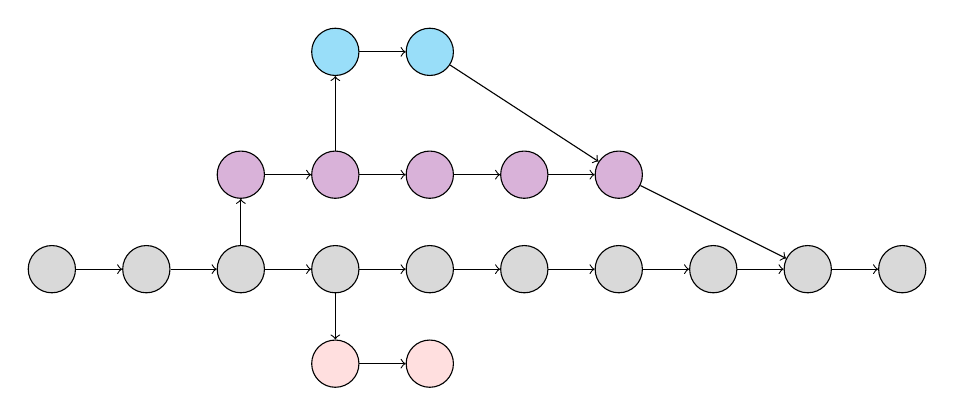
\begin{tikzpicture}[x=1.2cm, y=1.2cm, every node/.style={circle, draw, minimum size=6mm, inner sep=0pt}]

% Main branch nodes (10 total)
\foreach \x in {0,...,9}
    \node[fill=gray!30] (m\x) at (\x, 0) {};

% Edges for Main
\foreach \x in {0,...,8}
    \draw[->] (m\x) -- (m\the\numexpr\x+1\relax);

% Feature B (pastel pink)
\node[fill=pink!50] (b0) at (3, -1) {};
\node[fill=pink!50] (b1) at (4, -1) {};
\draw[->] (m3) -- (b0);
\draw[->] (b0) -- (b1);

% Feature A (pastel purple)
\node[fill=violet!30] (a0) at (2, 1) {};
\node[fill=violet!30] (a1) at (3, 1) {};
\node[fill=violet!30] (a2) at (4, 1) {};
\node[fill=violet!30] (a3) at (5, 1) {};
\node[fill=violet!30] (a4) at (6, 1) {};
\draw[->] (m2) -- (a0);
\draw[->] (a0) -- (a1);
\draw[->] (a1) -- (a2);
\draw[->] (a2) -- (a3);
\draw[->] (a3) -- (a4);
\draw[->] (a4) -- (m8);

% Feature A-1 (cornflower blue)
\node[fill=cyan!40] (a1a) at (3, 2.3) {};
\node[fill=cyan!40] (a1b) at (4, 2.3) {};
\draw[->] (a1) -- (a1a);
\draw[->] (a1a) -- (a1b);
\draw[->] (a1b) -- (a4);  % Merge into end of Feature A

\end{tikzpicture}
}

\vspace{1em}

\begin{center}
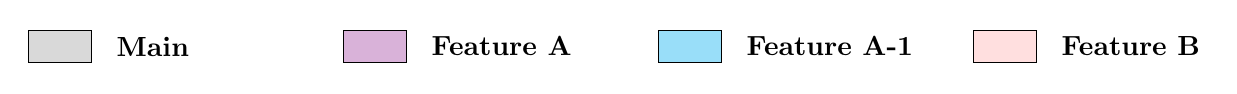
\begin{tikzpicture}[x=2cm, y=1cm]
    \draw[fill=gray!30]     (0,0) rectangle (0.4,0.4); \node[anchor=west] at (0.5,0.2) {\textbf{Main}};
    \draw[fill=violet!30]   (2,0) rectangle (2.4,0.4); \node[anchor=west] at (2.5,0.2) {\textbf{Feature A}};
    \draw[fill=cyan!40]     (4,0) rectangle (4.4,0.4); \node[anchor=west] at (4.5,0.2) {\textbf{Feature A-1}};
    \draw[fill=pink!50]     (6,0) rectangle (6.4,0.4); \node[anchor=west] at (6.5,0.2) {\textbf{Feature B}};
\end{tikzpicture}
\end{center}

\subsubsection{Local and Remote Repositories}

Version control in Git distinguishes between two primary types of repositories: local and remote. Understanding their relationship is fundamental to managing workflow and collaboration effectively.

\paragraph*{Local Repository}
A local repository exists on the developer's machine and includes the full history of commits, branches, and configuration files. It enables complete version control functionality without requiring a network connection.

\begin{itemize}
    \item Accessible only to the user of the local machine.
    \item Supports full Git operations such as commit, branch, revert, and diff.
    \item Local changes remain private until explicitly shared with others.
\end{itemize}

\paragraph*{Remote Repository}
A remote repository is hosted on an external server or cloud platform (e.g., GitHub, GitLab, Bitbucket). It serves as a shared version of the project that can be accessed by authorised collaborators.

\begin{itemize}
    \item Enables cloning, pushing, and pulling across distributed teams.
    \item Serves as a central copy for collaboration, backup, and integration.
    \item Updates made locally are only reflected on the remote when pushed.
\end{itemize}

\noindent\textit{\textbf{Note:} Local changes do not affect the remote repository until a \codecmd{git push} operation is performed. This separation allows developers to prepare and test changes independently before sharing them.}

\subsubsection{The Git Lifecycle}

Git operations follow a structured lifecycle that separates untracked changes from versioned history. The diagram below illustrates the primary phases and transitions in the Git workflow:

\begin{center}
\resizebox{\textwidth}{!}{
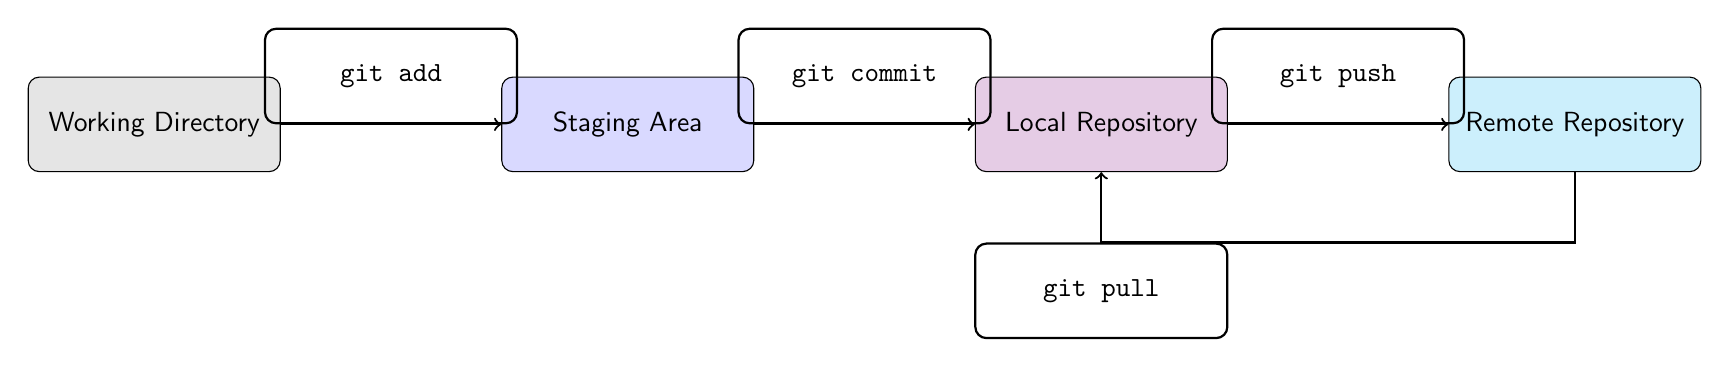
\begin{tikzpicture}[
    node distance=2.5cm and 2.8cm,
    every node/.style={rectangle, draw, rounded corners, minimum height=1.2cm, minimum width=3.2cm, font=\sffamily},
    arrow/.style={->, thick}
]

% Nodes
\node (wd)    [fill=gray!20]                  {Working Directory};
\node (stg)   [fill=blue!15, right=of wd]     {Staging Area};
\node (local) [fill=violet!20, right=of stg]  {Local Repository};
\node (remote)[fill=cyan!20, right=of local]  {Remote Repository};

% Arrows
\draw[arrow] (wd) -- node[above]{\texttt{git add}} (stg);
\draw[arrow] (stg) -- node[above]{\texttt{git commit}} (local);
\draw[arrow] (local) -- node[above]{\texttt{git push}} (remote);
\draw[arrow] (remote) -- ++(0,-1.5) -| node[below]{\texttt{git pull}} (local);

\end{tikzpicture}
}
\end{center}

This lifecycle ensures changes are intentionally managed at each step, promoting a clear separation between uncommitted, committed, and shared code states.

\subsubsection{Good Coding Practice with Version Control}

Version control systems such as Git are not only essential for collaboration and tracking changes, but also provide a platform to demonstrate and enforce good software development practices. Adhering to disciplined workflows can significantly enhance code quality, team productivity, and maintainability.

Some key practices include:

\begin{itemize}
    \item \textbf{Regular commits with meaningful messages}: Frequent commits that reflect logical units of work help create a clear project history. Commit messages should accurately summarise the change and follow a consistent style.
    
    \item \textbf{Code reviews through Pull Requests}: When using platforms like GitHub or GitLab, pull requests enable peer review, improve code quality, and foster knowledge sharing within a team.
    
    \item \textbf{Branch-based feature development}: New features or bug fixes should be developed in isolated branches. This reduces the risk of conflicts and allows multiple team members to work in parallel.
    
    \item \textbf{Refactoring and use of design patterns}: Although covered in detail in later topics, incorporating well-known design patterns and regular code refactoring into the version-controlled workflow contributes to long-term project scalability and readability.
\end{itemize}

Incorporating these practices into daily development workflows fosters a more structured, professional, and collaborative environment.

\subsubsection{Pull Requests with GitHub}

A pull request (PR) is a mechanism provided by platforms such as GitHub to propose, discuss, and review changes before merging them into a target branch. It serves as a formal code review process and facilitates collaboration among contributors.

The typical workflow involves the following steps:

\begin{enumerate}
    \item A contributor creates a new branch from the \texttt{main} branch or another base branch.
    \item Commits are made to this branch, encapsulating a single feature, bug fix, or improvement.
    \item Once complete, a pull request is opened on the GitHub repository, targeting the original branch (usually \texttt{main}).
    \item Reviewers can examine the changes, leave comments, request revisions, and ultimately approve or reject the changes.
    \item Once approved, the pull request is merged, integrating the proposed changes into the base branch.
\end{enumerate}

Pull requests support features such as inline code comments, status checks, automatic merge conflict detection, and enforcement of branch protection rules. This structured process helps maintain code quality, promotes accountability, and provides a documented history of the discussion surrounding each change.

\medskip
\textit{\textbf{Note}: While GitHub is the most widely used platform for pull requests, similar workflows are also available on GitLab, Bitbucket, and Azure DevOps.}



\subsection{Fundamental Git Commands}

This section outlines the most commonly used Git commands for managing source code, tracking changes, and collaborating with remote repositories. These commands form the foundation of most Git workflows.

\subsubsection{Initialising a Repository}

To create a new Git repository in the current directory:

\begin{tcolorbox}[colback=mintgreen, colframe=green!40!black, boxrule=0.5pt, sharp corners]
\begin{minted}[fontsize=\small]{bash}
git init
\end{minted}
\end{tcolorbox}

\noindent This sets up a new local repository by creating a \codecmd{.git} directory containing all version control metadata.

\subsubsection{Cloning a Repository}

To create a local copy of an existing remote repository:

\begin{tcolorbox}[colback=mintgreen, colframe=green!40!black, boxrule=0.5pt, sharp corners]
\begin{minted}[fontsize=\small]{bash}
git clone https://github.com/example/project.git
\end{minted}
\end{tcolorbox}

\noindent This creates a local folder containing the entire commit history and working directory from the remote source.

\subsubsection{Checking Repository Status}

To check which files have been modified, staged, or remain untracked:

\begin{tcolorbox}[colback=mintgreen, colframe=green!40!black, boxrule=0.5pt, sharp corners]
\begin{minted}[fontsize=\small]{bash}
git status
\end{minted}
\end{tcolorbox}

\noindent This is useful before staging or committing to verify the current state of the working directory.

\subsubsection{Staging Changes}

To stage a file for commit:

\begin{tcolorbox}[colback=mintgreen, colframe=green!40!black, boxrule=0.5pt, sharp corners]
\begin{minted}[fontsize=\small]{bash}
git add filename.java
\end{minted}
\end{tcolorbox}

\noindent To stage all changes in the current directory:

\begin{tcolorbox}[colback=mintgreen, colframe=green!40!black, boxrule=0.5pt, sharp corners]
\begin{minted}[fontsize=\small]{bash}
git add .
\end{minted}
\end{tcolorbox}

\noindent Staged files are added to the index (staging area) and will be included in the next \codecmd{commit}.

\subsubsection{Committing Changes}

To create a snapshot of staged changes:

\begin{tcolorbox}[colback=mintgreen, colframe=green!40!black, boxrule=0.5pt, sharp corners]
\begin{minted}[fontsize=\small]{bash}
git commit -m "Add user authentication module"
\end{minted}
\end{tcolorbox}

\noindent This saves the changes to the local repository history with a message describing the update.

\subsubsection{Viewing Commit History}

To view the list of previous commits:

\begin{tcolorbox}[colback=mintgreen, colframe=green!40!black, boxrule=0.5pt, sharp corners]
\begin{minted}[fontsize=\small]{bash}
git log
\end{minted}
\end{tcolorbox}

\noindent To view a more concise summary:

\begin{tcolorbox}[colback=mintgreen, colframe=green!40!black, boxrule=0.5pt, sharp corners]
\begin{minted}[fontsize=\small]{bash}
git log --oneline
\end{minted}
\end{tcolorbox}

\subsubsection{Inspecting Differences}

To view the changes in modified files (compared to last commit):

\begin{tcolorbox}[colback=mintgreen, colframe=green!40!black, boxrule=0.5pt, sharp corners]
\begin{minted}[fontsize=\small]{bash}
git diff
\end{minted}
\end{tcolorbox}

\noindent To compare staged changes to the last commit:

\begin{tcolorbox}[colback=mintgreen, colframe=green!40!black, boxrule=0.5pt, sharp corners]
\begin{minted}[fontsize=\small]{bash}
git diff --cached
\end{minted}
\end{tcolorbox}

\subsubsection{Pushing to a Remote Repository}

To upload local commits to the remote repository:

\begin{tcolorbox}[colback=mintgreen, colframe=green!40!black, boxrule=0.5pt, sharp corners]
\begin{minted}[fontsize=\small]{bash}
git push origin main
\end{minted}
\end{tcolorbox}

\noindent This updates the remote’s \codecmd{main} branch with all commits from the local repository using the \codecmd{push} command.

\subsubsection{Pulling from a Remote Repository}

To fetch and merge changes from the remote:

\begin{tcolorbox}[colback=mintgreen, colframe=green!40!black, boxrule=0.5pt, sharp corners]
\begin{minted}[fontsize=\small]{bash}
git pull origin main
\end{minted}
\end{tcolorbox}

\noindent This ensures the local branch is up to date with the remote by using the \codecmd{pull} command.

\subsubsection{Creating and Switching Branches}

To create a new branch called, for example, \codecmd{feature-login}:

\begin{tcolorbox}[colback=mintgreen, colframe=green!40!black, boxrule=0.5pt, sharp corners]
\begin{minted}[fontsize=\small]{bash}
git branch feature-login
\end{minted}
\end{tcolorbox}

\noindent To switch to that branch:

\begin{tcolorbox}[colback=mintgreen, colframe=green!40!black, boxrule=0.5pt, sharp corners]
\begin{minted}[fontsize=\small]{bash}
git checkout feature-login
\end{minted}
\end{tcolorbox}

\noindent To create and switch in one step:

\begin{tcolorbox}[colback=mintgreen, colframe=green!40!black, boxrule=0.5pt, sharp corners]
\begin{minted}[fontsize=\small]{bash}
git checkout -b feature-login
\end{minted}
\end{tcolorbox}

\subsubsection{Checking Branches}

To list all local branches:

\begin{tcolorbox}[colback=mintgreen, colframe=green!40!black, boxrule=0.5pt, sharp corners]
\begin{minted}[fontsize=\small]{bash}
git branch
\end{minted}
\end{tcolorbox}

\noindent To list local and remote branches:

\begin{tcolorbox}[colback=mintgreen, colframe=green!40!black, boxrule=0.5pt, sharp corners]
\begin{minted}[fontsize=\small]{bash}
git branch -a
\end{minted}
\end{tcolorbox}

\subsubsection{Origin}

The term \codecmd{origin} is a conventional name used to refer to the remote repository that a local repository is connected to. This association allows developers to push and pull updates with ease.

\begin{itemize}
    \item The name \codecmd{origin} is automatically assigned when a repository is cloned.
    \item If the local repository was not cloned, the remote must be manually added using the following command:
\end{itemize}

\begin{tcolorbox}[colback=mintgreen, colframe=green!40!black, boxrule=0.5pt, sharp corners]
\begin{minted}[fontsize=\small]{bash}
git remote add origin https://github.com/yourusername/your-repositoryname
\end{minted}
\end{tcolorbox}

\noindent Once added, the remote repository can be referenced using \codecmd{origin} in future commands such as \codecmd{git push origin main} or \codecmd{git pull origin main}. This configuration only needs to be performed once.

\subsection{JavaFX \& CRUD Application Development}

JavaFX is a set of Java libraries designed to support modern graphical user interface (GUI) development. It enables the creation of desktop applications with structured UI design, CSS-based styling, and event-driven control through Java code. JavaFX projects typically separate layout, behaviour, and appearance using FXML, controller classes, and stylesheets.

\subsubsection{JavaFX Structure and Components}

A JavaFX application is composed of three core layers:

\begin{itemize}
    \item \textbf{FXML}: An XML-based language used to define the layout of user interface elements in a declarative format.
    \item \textbf{CSS}: Cascading Style Sheets (.css) are used to style components visually (e.g., fonts, colours, spacing).
    \item \textbf{JavaFX Library}: Java classes handle event-driven logic and user interaction via a designated controller.
\end{itemize}

The following is a minimal example of a UI layout written in FXML:

\begin{minted}[fontsize=\small, linenos]{xml}
<VBox alignment="CENTER" spacing="20.0" xmlns:fx="http://javafx.com/fxml"
      fx:controller="com.example.addressbook.HelloController">
    <padding>
        <Insets top="20.0" right="20.0" bottom="20.0" left="20.0"/>
    </padding>
    <Label fx:id="welcomeText"/>
    <Button text="Hello!" onAction="#onHelloButtonClick"/>
</VBox>
\end{minted}

This layout defines a vertical box (VBox) aligned to the centre with a label and button. The controller class \codecmd{HelloController} manages button actions in Java.

\subsubsection{Stages, Scenes, and Controls}

JavaFX separates content and visual structure into well-defined concepts:

\begin{itemize}
    \item \textbf{Stage}: The top-level container that represents a window in a JavaFX application.
    \item \textbf{Scene}: A container that holds the visual content for a stage. Only one scene can be active on a stage at any time.
    \item \textbf{Controls}: Interactive GUI elements such as buttons, text fields, menus, and tables.
\end{itemize}

Example controls in JavaFX include:

\begin{itemize}
    \item \textbf{Button, ToggleButton, RadioButton}
    \item \textbf{TextField, TextArea, PasswordField}
    \item \textbf{ChoiceBox, ListView, TableView}
    \item \textbf{Slider, Tooltip, MenuBar}
\end{itemize}

These controls are instantiated in FXML and linked to event handlers defined in the controller.

\subsubsection{Creating a Basic Address Book (CRUD Operations)}

A CRUD-based address book allows users to:

\begin{itemize}
    \item \textbf{Create} a new contact record.
    \item \textbf{Read} or display contact entries in a view such as \codecmd{TableView}.
    \item \textbf{Update} existing records with new data.
    \item \textbf{Delete} entries from the dataset.
\end{itemize}

The controller manages logic for handling input events, validating form fields, and updating the user interface in response to changes.

A minimal FXML layout might include:

\begin{minted}[fontsize=\small, linenos]{xml}
<GridPane fx:controller="com.example.addressbook.AddressBookController"
          xmlns:fx="http://javafx.com/fxml" hgap="10" vgap="10">
    <Label text="Name:" GridPane.rowIndex="0" GridPane.columnIndex="0"/>
    <TextField fx:id="nameField" GridPane.rowIndex="0" GridPane.columnIndex="1"/>

    <Label text="Phone:" GridPane.rowIndex="1" GridPane.columnIndex="0"/>
    <TextField fx:id="phoneField" GridPane.rowIndex="1" GridPane.columnIndex="1"/>

    <Button text="Add Contact" onAction="#addContact"
            GridPane.rowIndex="2" GridPane.columnIndex="0"/>
    <Button text="Update" onAction="#updateContact"
            GridPane.rowIndex="2" GridPane.columnIndex="1"/>
    <Button text="Delete" onAction="#deleteContact"
            GridPane.rowIndex="2" GridPane.columnIndex="2"/>

    <TableView fx:id="contactTable" GridPane.rowIndex="3" GridPane.columnSpan="3"/>
</GridPane>
\end{minted}

In the controller class \codecmd{AddressBookController}, logic would be written to handle each operation:

\begin{minted}[fontsize=\small, linenos]{java}
public void addContact() {
    String name = nameField.getText();
    String phone = phoneField.getText();
    contactList.add(new Contact(name, phone));
}

public void updateContact() {
    Contact selected = contactTable.getSelectionModel().getSelectedItem();
    selected.setName(nameField.getText());
    selected.setPhone(phoneField.getText());
    contactTable.refresh();
}

public void deleteContact() {
    Contact selected = contactTable.getSelectionModel().getSelectedItem();
    contactList.remove(selected);
}
\end{minted}

\noindent This provides a full cycle for managing contact data within a GUI-based desktop application using JavaFX.

\medskip
\textit{\textbf{Note}: To persist data between sessions, the application may be extended with file I/O or a database backend in future implementations.}

\subsection{JavaFX Controls}

\subsubsection{Button}

A \codecmd{Button} in JavaFX is used to trigger actions in response to user interaction.

\begin{minted}[fontsize=\small]{java}
// Create a button with display text
Button button = new Button("Click Me");

// Set the button's action handler
button.setOnAction(e -> System.out.println("Button clicked"));
\end{minted}

To use a button:
\begin{itemize}
    \item Ensure it is added to a layout container (e.g., \codecmd{VBox}, \codecmd{HBox}).
    \item Include the layout in the \codecmd{Scene}.
    \item Display the scene in the \codecmd{Stage}.
\end{itemize}

\subsubsection{Text Field}

A \codecmd{TextField} is used to accept single-line user input.

\begin{minted}[fontsize=\small]{java}
// Create a text field with placeholder text
TextField textField = new TextField();
textField.setPromptText("Enter your name");
\end{minted}

\noindent To retrieve input:
\begin{minted}[fontsize=\small]{java}
String input = textField.getText();
\end{minted}

Ensure the text field is added to a layout and displayed in a scene.

\subsubsection{List View}

A \codecmd{ListView} displays a vertical list of selectable items.

\begin{minted}[fontsize=\small]{java}
ListView<String> listView = new ListView<>();
listView.getItems().addAll("Apple", "Banana", "Cherry");
\end{minted}

\noindent To get the selected item:
\begin{minted}[fontsize=\small]{java}
String selected = listView.getSelectionModel().getSelectedItem();
\end{minted}

\subsubsection{List View}

A \codecmd{ListView} displays a vertical list of selectable items.

\begin{minted}[fontsize=\small]{java}
ListView<String> listView = new ListView<>();
listView.getItems().addAll("Apple", "Banana", "Cherry");
\end{minted}

\noindent To get the selected item:
\begin{minted}[fontsize=\small]{java}
String selected = listView.getSelectionModel().getSelectedItem();
\end{minted}

\subsubsection{Table View}

A \codecmd{TableView} displays structured data in rows and columns.

\begin{minted}[fontsize=\small]{java}
TableView<Person> table = new TableView<>();

TableColumn<Person, String> first = new TableColumn<>("First Name");
first.setCellValueFactory(new PropertyValueFactory<>("firstName"));

TableColumn<Person, String> last = new TableColumn<>("Last Name");
last.setCellValueFactory(new PropertyValueFactory<>("lastName"));

table.getColumns().addAll(first, last);
\end{minted}

\noindent This requires a model class:
\begin{minted}[fontsize=\small]{java}
public class Person {
    private final String firstName;
    private final String lastName;

    public Person(String f, String l) {
        this.firstName = f;
        this.lastName = l;
    }

    public String getFirstName() { return firstName; }
    public String getLastName() { return lastName; }
}
\end{minted}

\subsubsection{Tooltip}

Tooltips display extra information when hovering over a control.

\begin{minted}[fontsize=\small]{java}
TextField field = new TextField();
Tooltip tooltip = new Tooltip("Must be at least 8 characters");
field.setTooltip(tooltip);
\end{minted}

\subsubsection{Choice Box}

A \codecmd{ChoiceBox} allows the user to select one item from a dropdown list.

\begin{minted}[fontsize=\small]{java}
ChoiceBox<String> choiceBox = new ChoiceBox<>();
choiceBox.getItems().addAll("Red", "Green", "Blue");
choiceBox.setValue("Green");
\end{minted}

\noindent To get the selected value:
\begin{minted}[fontsize=\small]{java}
String colour = choiceBox.getValue();
\end{minted}

\subsubsection{Choice Box}

A \codecmd{ChoiceBox} allows the user to select one item from a dropdown list.

\begin{minted}[fontsize=\small]{java}
ChoiceBox<String> choiceBox = new ChoiceBox<>();
choiceBox.getItems().addAll("Red", "Green", "Blue");
choiceBox.setValue("Green");
\end{minted}

\noindent To get the selected value:
\begin{minted}[fontsize=\small]{java}
String colour = choiceBox.getValue();
\end{minted}

\subsubsection{Toggle Button}

A \codecmd{ToggleButton} can be switched on or off.

\begin{minted}[fontsize=\small]{java}
ToggleButton toggle = new ToggleButton("Activate");
toggle.setSelected(true); // start in active state
\end{minted}

\subsubsection{Radio Button}

\codecmd{RadioButton}s are used in groups where only one can be selected at a time.

\begin{minted}[fontsize=\small]{java}
RadioButton r1 = new RadioButton("Option A");
RadioButton r2 = new RadioButton("Option B");

ToggleGroup group = new ToggleGroup();
r1.setToggleGroup(group);
r2.setToggleGroup(group);
r1.setSelected(true); // default selection
\end{minted}

\subsubsection{Slider}

A \codecmd{Slider} allows the user to select a numeric value within a range.

\begin{minted}[fontsize=\small]{java}
Slider slider = new Slider(0, 100, 50); // min, max, initial value
slider.setShowTickMarks(true);
slider.setShowTickLabels(true);
\end{minted}

To read the current value:
\begin{minted}[fontsize=\small]{java}
double value = slider.getValue();
\end{minted}

\subsubsection{Menu Bar}

A \codecmd{MenuBar} provides a menu interface at the top of a window.

\begin{minted}[fontsize=\small]{java}
MenuBar menuBar = new MenuBar();

Menu fileMenu = new Menu("File");
MenuItem exitItem = new MenuItem("Exit");
exitItem.setOnAction(e -> System.exit(0));

fileMenu.getItems().add(exitItem);
menuBar.getMenus().add(fileMenu);
\end{minted}


\subsection{JavaFX Packages}

JavaFX is organised into modular packages that separate functionality by component type. This modular design enables developers to import only what is necessary for their application, improving clarity and efficiency.

A commonly used package is \codecmd{javafx.scene}, which provides core UI classes such as \codecmd{Scene}, \codecmd{Node}, and layout controls. Within this structure, additional subpackages offer specialised capabilities for different domains.

One such example is the \codecmd{javafx.scene.chart} package, included in the base JavaFX library. It provides a suite of classes for creating chart-based data visualisations, including:

\begin{itemize}
    \item \codecmd{LineChart}, \codecmd{BarChart}, \codecmd{PieChart}
    \item \codecmd{XYChart}, \codecmd{CategoryAxis}, \codecmd{NumberAxis}
\end{itemize}

These chart classes integrate with the JavaFX scene graph and can be embedded within UI layouts like any other control. They support dynamic updates, style customisation, and data-driven rendering.

\medskip
\textit{Other useful JavaFX packages include \codecmd{javafx.scene.control}, \codecmd{javafx.stage}, and \codecmd{javafx.fxml}.}

\subsubsection{Example: Line Chart in JavaFX}

The following example demonstrates how to create a basic \codecmd{LineChart} in JavaFX using the \codecmd{javafx.scene.chart} package.

\begin{minted}[fontsize=\small, linenos, breaklines]{java}
import javafx.application.Application;
import javafx.scene.Scene;
import javafx.scene.chart.*;
import javafx.scene.layout.VBox;
import javafx.stage.Stage;

public class LineChartExample extends Application {

    @Override
    public void start(Stage stage) {
        stage.setTitle("Line Chart Example");

        // Define axes
        NumberAxis xAxis = new NumberAxis();
        NumberAxis yAxis = new NumberAxis();
        xAxis.setLabel("Time");
        yAxis.setLabel("Value");

        // Create line chart
        LineChart<Number, Number> lineChart = new LineChart<>(xAxis, yAxis);
        lineChart.setTitle("Sample Data Over Time");

        // Create data series
        XYChart.Series<Number, Number> series = new XYChart.Series<>();
        series.setName("Sensor A");

        // Add data points
        series.getData().add(new XYChart.Data<>(0, 23));
        series.getData().add(new XYChart.Data<>(1, 14));
        series.getData().add(new XYChart.Data<>(2, 15));
        series.getData().add(new XYChart.Data<>(3, 24));
        series.getData().add(new XYChart.Data<>(4, 34));
        series.getData().add(new XYChart.Data<>(5, 36));

        lineChart.getData().add(series);

        // Display chart
        VBox root = new VBox(lineChart);
        Scene scene = new Scene(root, 600, 400);
        stage.setScene(scene);
        stage.show();
    }

    public static void main(String[] args) {
        launch();
    }
}
\end{minted}

This example creates a line chart with two numerical axes and plots a single data series. The chart is displayed in a JavaFX \codecmd{Stage} using a \codecmd{VBox} layout.

\subsection{JavaFX Layout Panes}

JavaFX provides several layout containers (panes) to help structure and organise components in a user interface. Each pane arranges child nodes according to a specific layout strategy. Below are examples of common layout panes:

\paragraph{\textbf{VBox}}

A vertical box layout. Arranges elements from top to bottom.
\begin{minted}[fontsize=\small]{java}
VBox vbox = new VBox(10); // spacing of 10 pixels
vbox.getChildren().addAll(new Button("One"), new Button("Two"));
\end{minted}

\paragraph{\textbf{HBox}}

A horizontal box layout. Arranges elements from left to right.
\begin{minted}[fontsize=\small]{java}
HBox hbox = new HBox(10);
hbox.getChildren().addAll(new Label("Name:"), new TextField());
\end{minted}

\paragraph{\textbf{Tile Pane}}

Places components in uniformly sized tiles.
\begin{minted}[fontsize=\small]{java}
TilePane tile = new TilePane();
tile.getChildren().addAll(new Button("A"), new Button("B"), new Button("C"));
\end{minted}

\paragraph{\textbf{Grid Pane}}

Lays out components in a flexible grid of rows and columns.
\begin{minted}[fontsize=\small]{java}
GridPane grid = new GridPane();
grid.add(new Label("Username:"), 0, 0);
grid.add(new TextField(), 1, 0);
\end{minted}

\paragraph{\textbf{Border Pane}}

Divides space into five regions: top, bottom, left, right, and center.
\begin{minted}[fontsize=\small]{java}
BorderPane border = new BorderPane();
border.setTop(new Label("Header"));
border.setCenter(new TextArea());
\end{minted}

\paragraph{\textbf{Flow Pane}}

Lays out children in a flow that wraps at the boundary.
\begin{minted}[fontsize=\small]{java}
FlowPane flow = new FlowPane();
flow.getChildren().addAll(new Button("One"), new Button("Two"), new Button("Three"));
\end{minted}

\paragraph{\textbf{Stack Pane}}

Stacks children on top of each other.
\begin{minted}[fontsize=\small]{java}
StackPane stack = new StackPane();
stack.getChildren().addAll(new Rectangle(100, 100), new Label("Overlay"));
\end{minted}

\paragraph{\textbf{Anchor Pane}}

Positions children at fixed distances from the pane's edges.
\begin{minted}[fontsize=\small]{java}
AnchorPane anchor = new AnchorPane();
Button btn = new Button("Anchored");
AnchorPane.setTopAnchor(btn, 10.0);
AnchorPane.setLeftAnchor(btn, 20.0);
anchor.getChildren().add(btn);
\end{minted}

\subsection{WYSIWYG Editors and Scene Builder}

\textbf{WYSIWYG} stands for \textit{What You See Is What You Get}. These tools allow users to manipulate content visually, rather than writing code directly. A common example outside programming is WordPress.

WYSIWYG editors are useful for beginners, as they reduce the barrier to entry by allowing intuitive drag-and-drop design. However, they often limit fine-grained control or introduce complexity when making specific changes without accessing the underlying code.

\medskip
\textbf{Scene Builder} is a popular WYSIWYG editor for constructing JavaFX graphical user interfaces. It enables the visual arrangement of nodes and layout panes, generating the corresponding FXML file automatically.

\begin{itemize}
    \item Scene Builder must be installed and configured separately.
    \item The Week 4 Practical focuses on writing and manipulating FXML directly without using Scene Builder.
\end{itemize}

\begin{figure}[H]
    \centering
    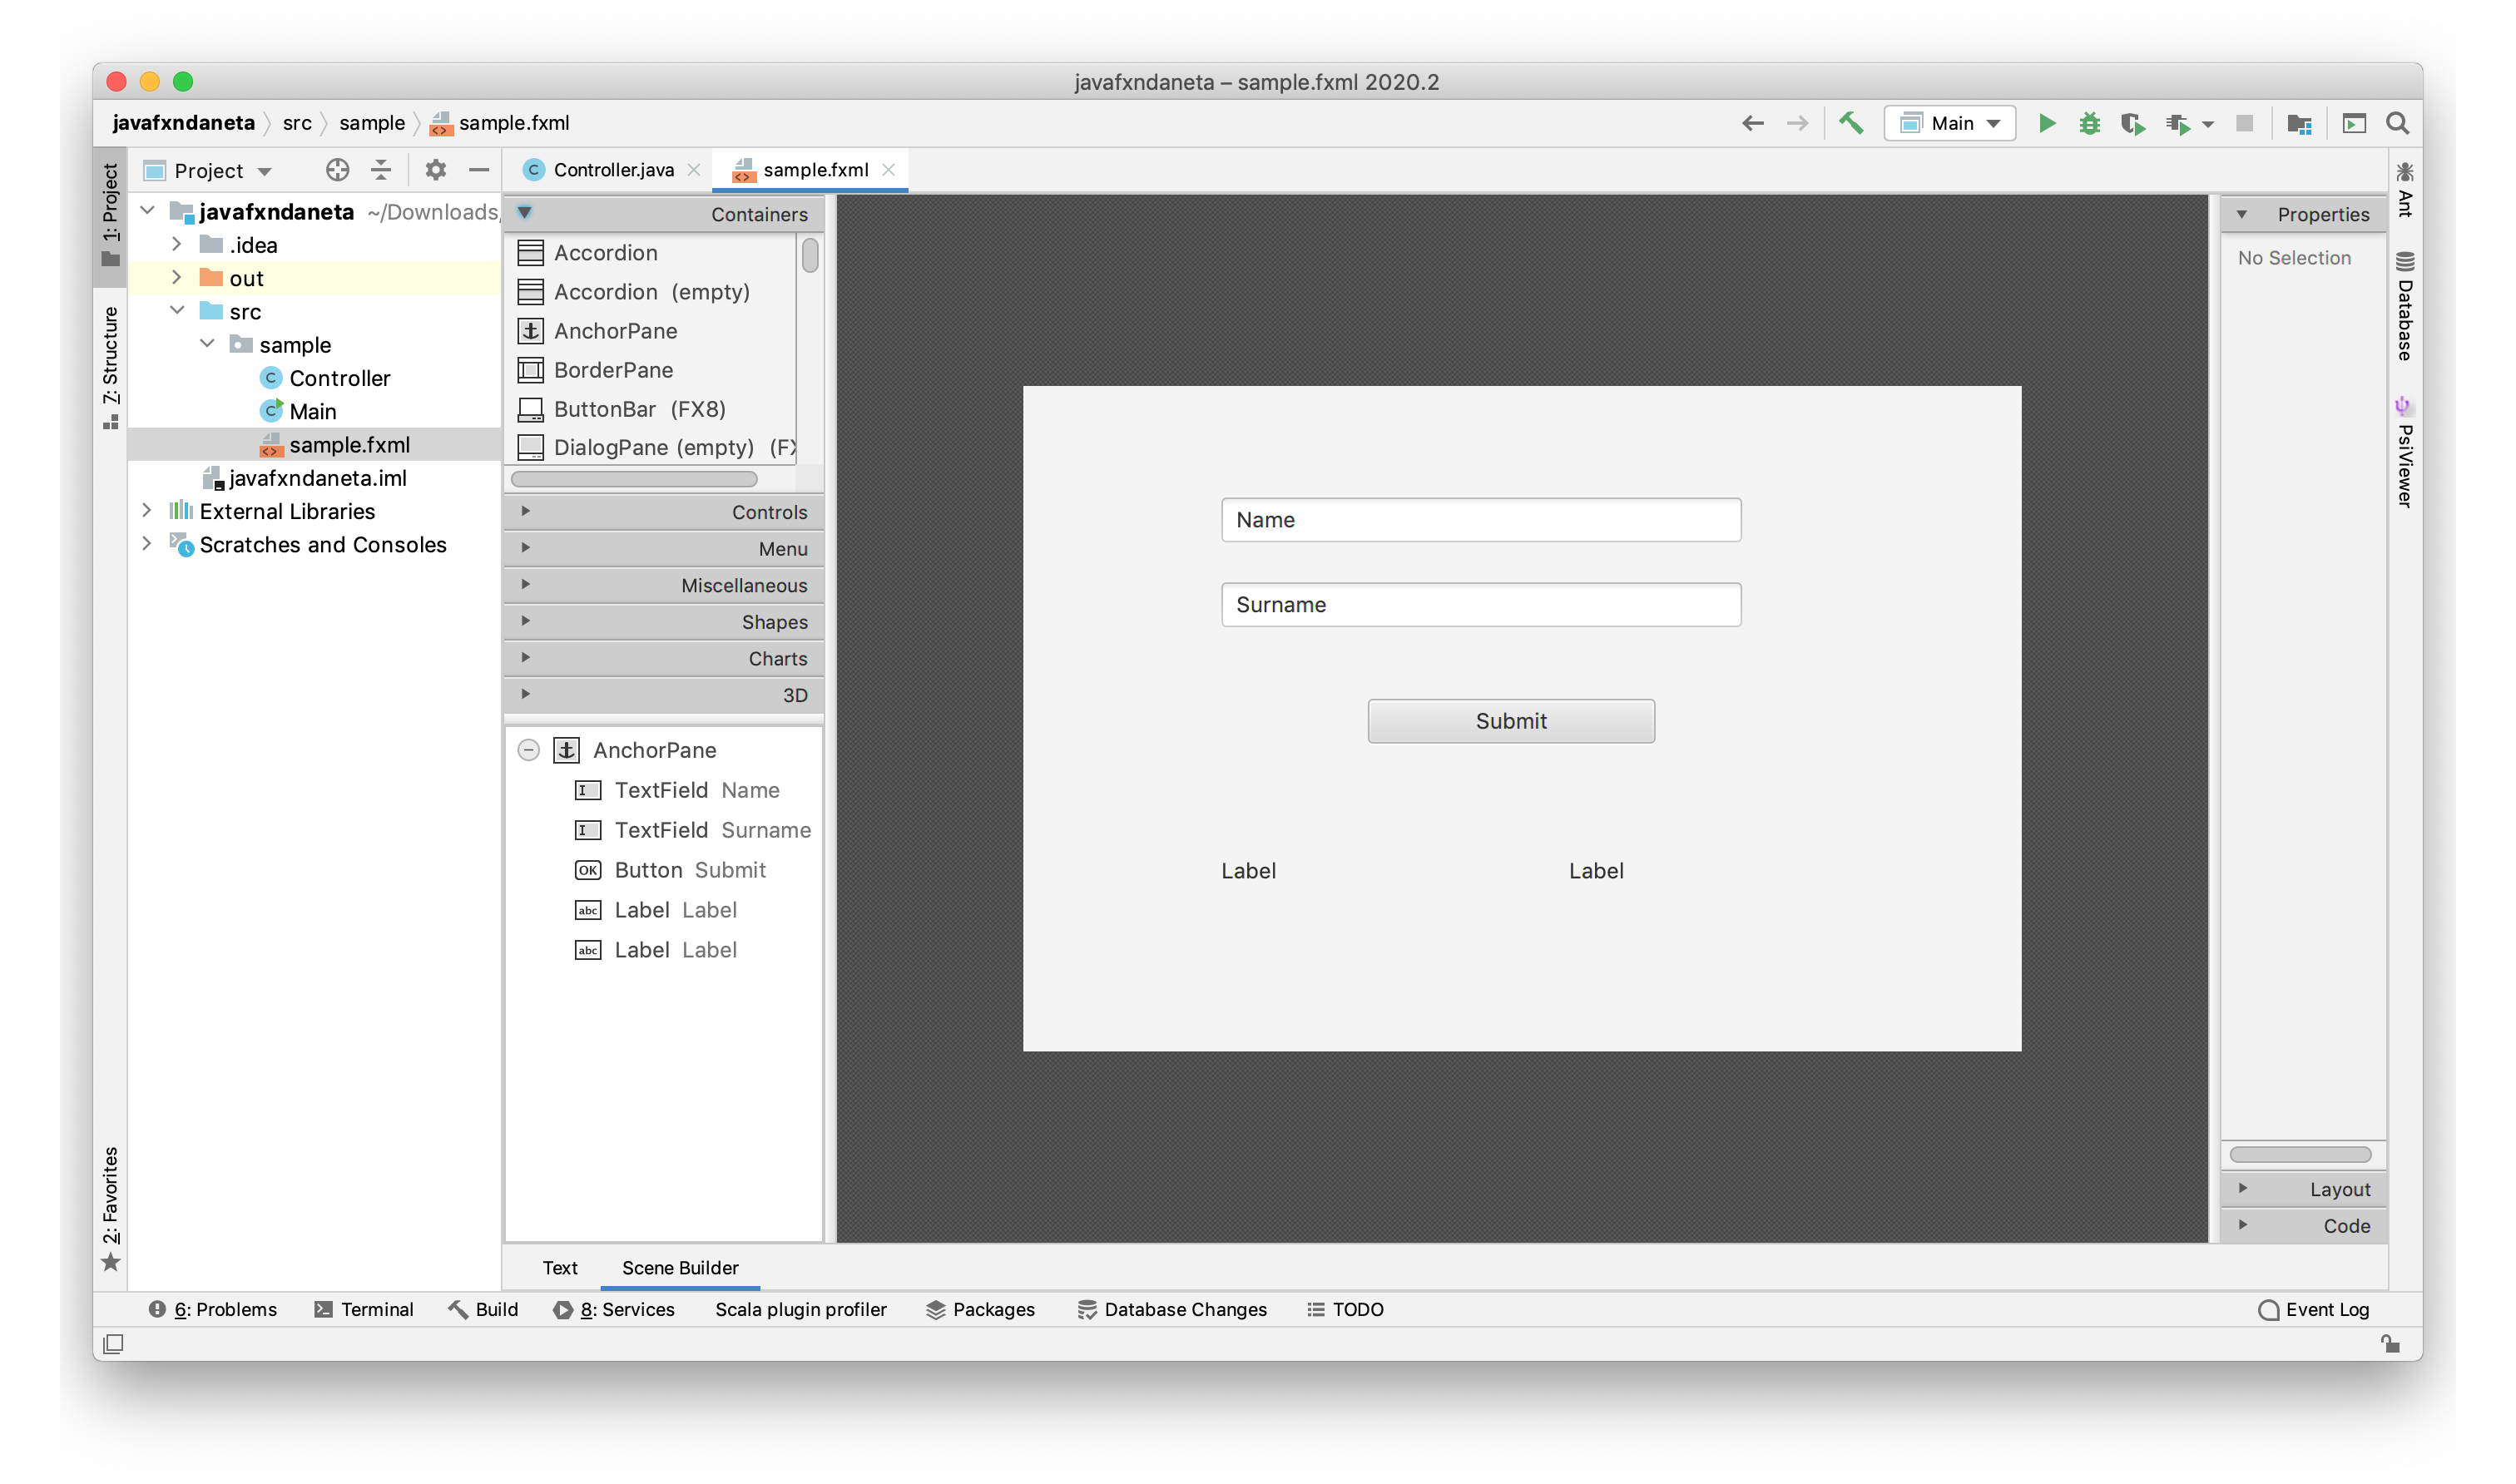
\includegraphics[width=0.9\textwidth]{scene-builder.png}
    \caption{Scene Builder WYSIWYG Interface in IntelliJ IDEA}
\end{figure}

\subsection{Fidelity in Prototyping}

Prototyping in software and interface design is a crucial step in conceptualising, evaluating, and iterating on design ideas. Prototypes can vary in fidelity depending on their purpose, ranging from rough sketches to polished interfaces.

\begin{figure}[h!]
\centering
\includegraphics[width=0.9\linewidth]{11.jpg}
\caption{Example of different prototype fidelity levels}
\label{fig:prototype-fidelity}
\end{figure}

\subsubsection{Low-Fidelity Prototypes}

Low-fidelity (lo-fi) prototypes are quick, inexpensive representations of design concepts, often created during the early stages of the design process.

\begin{itemize}
    \item Typically consist of hand-drawn sketches or simple diagrams.
    \item Focus on structure, layout, and overall user flow rather than visual style.
    \item Tools include pen and paper, whiteboards, or basic digital sketching apps.
    \item Sketching can often be more effective than digital tools such as Figma in early phases.
    \item Capturing sketches with a phone is recommended for record-keeping.
    \item Useful for gathering early feedback from stakeholders and team members.
\end{itemize}

\textbf{Benefits:}
\begin{itemize}
    \item Fast and easy to create.
    \item Encourages iteration and exploration.
    \item Reduces emotional attachment to designs.
    \item Supports collaborative design and brainstorming.
\end{itemize}

\subsubsection{Medium-Fidelity Prototypes}

Medium-fidelity (mid-fi) prototypes incorporate more detail than lo-fi versions and are often developed once the direction of the user interface becomes clearer.

\begin{itemize}
    \item Usually created with software such as Figma, Sketch, Balsamiq, or Wireframe tools.
    \item Include refined layout, basic navigation, and possibly placeholder text or icons.
    \item Allow simulation of user interactions (e.g., clicking through screens).
    \item Present a clearer structure of the product for feedback.
\end{itemize}

\textbf{Benefits:}
\begin{itemize}
    \item More accurate visual representation.
    \item Easier for clients or users to understand and evaluate.
    \item Enables early usability testing.
\end{itemize}

\subsubsection{High-Fidelity Prototypes}

High-fidelity (hi-fi) prototypes are close representations of the final product in both appearance and interactivity.

\begin{itemize}
    \item Created using advanced design tools or development platforms.
    \item Include real images, fonts, colours, and interactive elements.
    \item Behave like the final application (e.g., hover effects, form validation).
    \item Often used for stakeholder demonstrations or usability testing.
\end{itemize}

\textbf{Benefits:}
\begin{itemize}
    \item Provides realistic user experiences.
    \item Useful for stakeholder approval before development.
    \item Allows detailed testing of interaction flows.
    \item Can serve as a reference for developers.
\end{itemize}




\subsection{The Model-View-Controller (MVC) Pattern}

The Model-View-Controller (MVC) design pattern is one of the foundational patterns in object-oriented programming. Originally introduced by Trygve Reenskaug in the 1970s, it continues to be widely used in software design today.

\subsubsection{Core Components of MVC}
MVC divides application responsibilities into three distinct components:

\subsubsection*{The Model}
\begin{itemize}
\item \textbf{Data Management} – Responsible for handling and storing application data. It often interacts with databases and manages CRUD operations.
\item \textbf{Business Logic} – Executes the core functionality and rules of the application. This is where calculations and domain-specific operations occur.
\item \textbf{Data Validation} – Ensures the integrity and correctness of data before it is processed or stored.
\end{itemize}

\subsubsection*{The View}
\begin{itemize}
\item \textbf{Displays Data} – Presents information from the model in a visual and human-readable format.
\item \textbf{Captures User Input} – Receives user interactions (e.g., button clicks, text input) and forwards them to the controller.
\item \textbf{UI Updates} – Reflects any changes in the model by updating the interface dynamically. Commonly uses the Observer Pattern.
\end{itemize}

\subsubsection*{The Controller}
\begin{itemize}
\item \textbf{Request Processing} – Handles incoming events from the user or other parts of the system.
\item \textbf{Mediator} – Acts as an intermediary between the view and the model, updating one based on changes to the other.
\item \textbf{Session Management} – Manages session state in stateless applications by storing and retrieving context-specific data.
\end{itemize}

\subsubsection{MVC Lifecycle Diagram}

\begin{center}
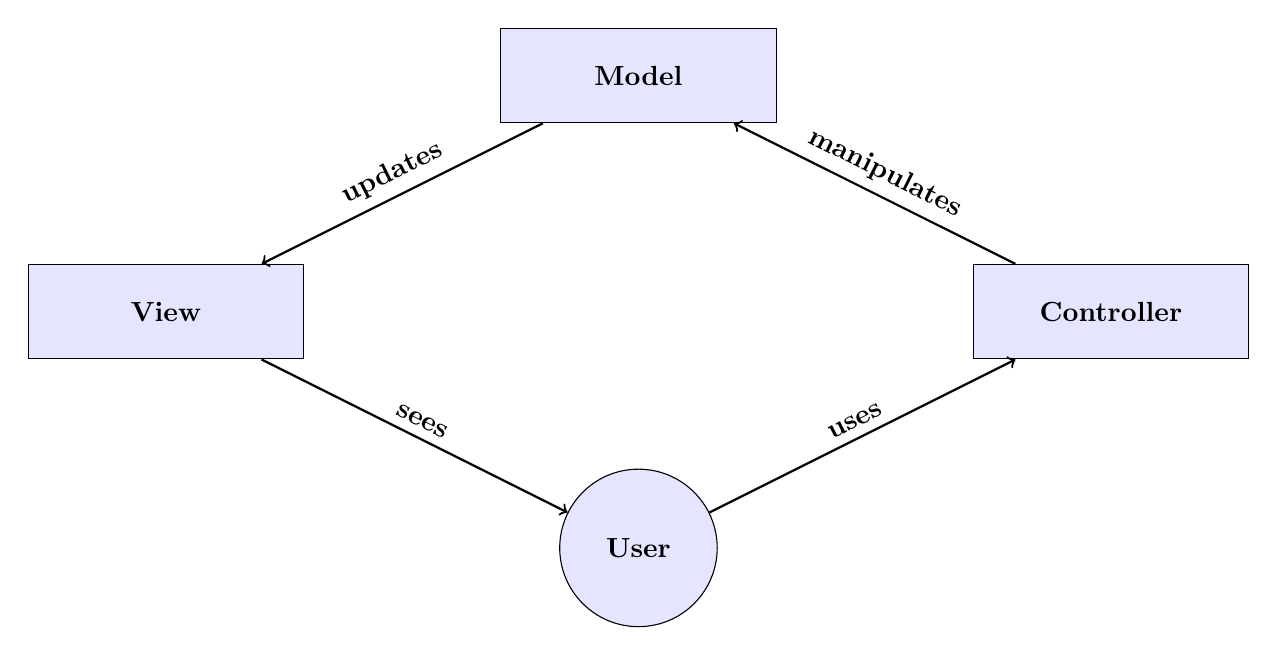
\begin{tikzpicture}[node distance=5cm, every node/.style={align=center}]
    % Node layout in circular form with reduced distance
    \node[draw, rectangle, fill=blue!10, minimum width=3.5cm, minimum height=1.2cm] (model) at (0, 6) {\textbf{Model}};
    \node[draw, rectangle, fill=blue!10, minimum width=3.5cm, minimum height=1.2cm] (view) at (-6, 3) {\textbf{View}};
    \node[draw, circle, fill=blue!10, minimum size=2cm] (user) at (0, 0) {\textbf{User}};
    \node[draw, rectangle, fill=blue!10, minimum width=3.5cm, minimum height=1.2cm] (controller) at (6, 3) {\textbf{Controller}};

    % Arrows with consistent lengths and labels
    \draw[->, thick] (model) -- node[sloped, above] {\textbf{updates}} (view);
    \draw[->, thick] (view) -- node[sloped, above] {\textbf{sees}} (user);
    \draw[->, thick] (user) -- node[sloped, above] {\textbf{uses}} (controller);
    \draw[->, thick] (controller) -- node[sloped, above] {\textbf{manipulates}} (model);
\end{tikzpicture}
\end{center}

\subsubsection{Purpose of MVC}

The primary purpose of MVC is to achieve \textbf{separation of concerns}, which facilitates:
\begin{itemize}
    \item \textbf{Testability} – Components can be tested independently.
    \item \textbf{Maintainability} – Easier to locate and fix issues.
    \item \textbf{Scalability} – Enhancements or extensions can be added with minimal impact.
    \item \textbf{Reusability} – Components can be reused across different applications.
\end{itemize}


 
















\subsection{The Integrated Build \& Javadoc}

\subsection{Refactoring \& Design Patterns}

\subsection{Threading and APIs}

% ===================================================================================
\newpage
\section{Software Development}

\subsection{High Performing Teams}

High-performing teams are built on trust, mutual accountability, commitment to shared goals, and open communication. Patrick Lencioni’s model, \textit{The Five Dysfunctions of a Team} (2002), identifies key behaviours that undermine effective teamwork. By recognising and addressing these dysfunctions, teams can establish healthier dynamics and enhance performance.

\subsubsection{What is a Team?}

A team is more than a group of individuals working together. According to Katzenbach and Smith:
\textit{\begin{quote}
“A team is a small number of people with complementary skills who are committed to a common purpose, set of performance goals, and an agreed approach for which they hold themselves mutually accountable.”
\end{quote}}

This definition highlights the importance of shared goals, accountability, and coordinated effort in building successful teams.

\subsubsection{Absence of Trust}

Trust is foundational to collaboration. A lack of trust often arises from the desire to protect one’s ego or to avoid appearing vulnerable, weak, or uninformed.

\textbf{Strategies to build trust:}
\begin{itemize}
    \item Encourage sharing of personal background and experience in a safe, respectful environment.
    \item Model vulnerability and openness to foster psychological safety.
    \item Promote mutual respect and demonstrate empathy in team interactions.
\end{itemize}

\subsubsection{Fear of Conflict}

Constructive conflict enables better decision-making and innovation. Avoiding conflict may stem from lack of psychological safety or fear of interpersonal tension.

\textbf{Strategies to encourage constructive conflict:}
\begin{itemize}
    \item Focus on the issue rather than the individual.
    \item Seek to understand different perspectives genuinely.
    \item Use calm, respectful language, and maintain composure.
    \item Set “productive debate” as a team norm early in group formation.
\end{itemize}

\subsubsection{Lack of Commitment}

Commitment falters when team members feel excluded from decision-making or when objectives are unclear.

\vspace{1em}
\textbf{Strategies to strengthen commitment:}
\begin{itemize}
    \item Ensure all voices are heard and considered before decisions are finalised.
    \item Record decisions and agreed actions clearly at every meeting.
    \item Adopt open conflict resolution as a team standard to prevent avoidance.
    \item Encourage individuals to confirm their agreement with action items explicitly.
\end{itemize}

\subsubsection{Avoidance of Accountability}

Accountability can be neglected when it is not embedded in team culture. A reluctance to challenge peers or address missed obligations undermines group standards.

\vspace{1em}
\textbf{Strategies to encourage accountability:}
\begin{itemize}
    \item Establish accountability as a team norm from the outset.
    \item Communicate openly about progress and flag issues early.
    \item Reinforce responsibility by following up on deadlines and actions.
    \item Welcome constructive feedback and express appreciation when held accountable.
\end{itemize}

\subsubsection{Inattention to Results}

When individual priorities take precedence over team outcomes, collective performance suffers. A results-focused mindset requires clarity and continuous reinforcement.

\vspace{1em}
\textbf{Strategies to focus on results:}
\begin{itemize}
    \item Clearly define team deliverables and standards at the beginning.
    \item Regularly revisit goals and progress in meetings.
    \item Monitor outcomes continuously and adjust actions as needed.
\end{itemize}

\subsubsection{Establishing Team Norms and Practices}

To foster a high-performing team environment, consider implementing the following:

\begin{itemize}
    \item Set clear deliverables, roles, and expectations for all members.
    \item Define communication protocols—who communicates, how, and when.
    \item Conduct structured meetings with agendas, action points, and follow-ups.
    \item Be transparent, goal-oriented, and consistent with deadlines.
    \item Encourage mutual support, open feedback, and shared responsibility.
\end{itemize}

\subsection{Agile \& Sprint Planning}

\subsection{Persistence}

\subsection{Test Driven Development}

\subsection{User Testing}


\end{document}
